\section{The Tool}
\label{sec:impl}
In our tool we present trips as dots moving on a black background.
Every dot can be colored blue (indicating bike share subscription of the driver)
or red (indicating a casual user). The dots move on a curved path from
its origin to its destination to avoid over-plotting of opposing trips
similar to Wood~\etal\cite{Wood2011} and
Beecham~\etal\cite{Beecham2012}.
However, they cycle the animation of a given set of trips continuously,
whereas we split the time in slices and advance time constantly.
In our approach the complete data set is split into time slices of equal
length and within those slices we define a relevant window.
At the beginning of each time slice we create dots for trips of the
relevant window and start moving them. If a trip lasts longer than the
relevant window we let it continue to move during the next slice.

To make the vast number of simultaneous trips for longer slices
easier to read we aggregate similar trips based on origin, destination,
duration, and type. The aggregated trips are then represented as larger
dot.
Furthermore, we show a trail for each moving dot to make its
route easier to follow and gasp.
The user can vary those parameters when needed and can also
set a threshold of a minimal number of trips for a dot to be shown at all.

In addition to the animated trails the tool shows a summary of
future slices as bar chart.
The bar chart shows the total number of trips in the relevant window
of the given slices.
It starts with the currently displayed slice and shows the next 59 slices.
The blue part of the bar shows the number of subscriber trips during
the relevant window and the red part shows the number of casual users.

As further information about the current state the start and end times
of the current relevant window is always shown.
The complete tool can be seen in Figure~\ref{fig:tool}.
It is efficiently implemented using a MySQL database as storage and
OpenGL accelerated image blending to show the movement of the dots
and simulate their trails.
This allows for an interactive user experience with immediate feedback.

\begin{figure}
\centering
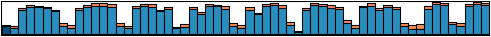
\includegraphics[width=\linewidth]{images/barchart.png}
\caption{The bar chart view showing the number of trips per relevant
window.
In this bar chart the slice length is one day, the relevant window is
during the morning rush hour.
Weekends can be easily identified by a decreasing number of trips
which sometimes start already on fridays.
The current (leftmost) slice is a Saturday.}
\label{fig:bar}
\end{figure}
